%%%%%%%%%%%%%%%%%%%%%%%%%%%%%%%%%%%%%%%%%
% Их сургуулийн оюутны тезис  
% LaTeX Загвар
% Version 2.3 (25/3/16)
%
% Энэ загвар нь дараах сайтаас авсан загварын монгол хувилбар юм.
% http://www.LaTeXTemplates.com
%
% Version 2.x major modifications by:
% Vel (vel@latextemplates.com)
%
% Анхдагч загварын эх үүсвэр:
% Steve Gunn (http://users.ecs.soton.ac.uk/srg/softwaretools/document/templates/)
% Sunil Patel (http://www.sunilpatel.co.uk/thesis-template/)
%
% Загварын лиценз:
% CC BY-NC-SA 3.0 (http://creativecommons.org/licenses/by-nc-sa/3.0/)
%
%%%%%%%%%%%%%%%%%%%%%%%%%%%%%%%%%%%%%%%%%

%-------------------------------------------------------------------------------
%	PACKAGES AND OTHER DOCUMENT CONFIGURATIONS
%-------------------------------------------------------------------------------

\documentclass[
12pt, % Баримтын фонтын хэмжээ, сонголт: 10pt, 11pt, 12pt
oneside, % Хоёр талаар хэвлэж үдэхээр тохируулсан. Нэг тал бол комментыг арилга
%chapterinoneline,% Нэг мөрөнд бүлгийн дугаар, нэрийг гаргах
english, % babel багцын хэлний тохиргоо
onehalfspacing, % Мөр хоорондын зай. Сонголтууд: singlespacing, onehalfspacing, doublespacing
%draft, % Ноорог горимд шилжихийн тулд комментыг арилга(зураг, холбоос, hboxes гарахгүй)
nolistspacing, % Хэрэв мөр хоорондын зай onehalfspacing эсвэл doublespacing бол, жагсаалтын мөр хоорондын зайг single болгохын тулд комментыг арилга
%liststotoc, % Зураг/хүснэгт/бусад жагсаалтыг гарчигт оруулахын тулд комментыг арилга
%toctotoc, % Uncomment to add the main table of contents to the table of contents
%parskip, % Параграф хооронд зай оруулахын тулд комментыг арилга
%nohyperref, % hyperref багцыг ачаалахгүй бол комментыг арилга
headsepline, % Толгой мөрийн доогуур шугам татахын тулд комментыг арилга
]{MUST-Thesis} % Энэ класс файл нь баримтын бүтцийг тодорхойлно

\usepackage[utf8]{inputenc} % Олон улсын тэмдэгт оруулахад хэрэгтэй
\usepackage[T2A]{fontenc} % Олон улсын тэмдэгтийн гаралтын кодчилол
\usepackage[mongolian]{babel}

\usepackage{titlesec}
\usepackage[table]{xcolor}
\usepackage{rotating} % эргүүлэх
\usepackage{enumitem}
\setlist{noitemsep}

\let\oldtabular\tabular
\let\endoldtabular\endtabular
\renewenvironment{tabular}
   {\bgroup\singlespacing\oldtabular}%
   {\endoldtabular\egroup}
\let\oldverse\verse
\let\endoldverse\endverse
\renewenvironment{verse}
   {\bgroup\singlespacing\oldverse}%
   {\endoldverse\egroup}

\usepackage{caption,longtable,ltcaption}
\DeclareCaptionJustification{nohyphen}{\hyphenpenalty=10000}
\captionsetup{justification=nohyphen}

\usepackage{pgf}
\usepackage{tikz} % зураг зурах
\usetikzlibrary{shapes,arrows,automata}

\definecolor{OliveGreen}{cmyk}{0.64,0,0.95,0.40}
\definecolor{CadetBlue}{cmyk}{0.62,0.57,0.23,0}
\definecolor{Cover}{RGB}{102,255,255}
\definecolor{Chapter}{RGB}{255,220,180}

\definecolor{lightlightgray}{gray}{0.9}
\usepackage{listings}
\renewcommand{\lstlistingname}{Эх код} % Програмын эх код хэвлэх
\lstset{
language=C,                             % Code langugage
basicstyle=\linespread{1.0}\ttfamily,                   % Code font
keywordstyle=\color{OliveGreen},        % Keywords font ('*' = uppercase)
commentstyle=\color{CadetBlue},         % Comments font
numbers=left,                           % Line nums position
numberstyle=\tiny,                      % Line-numbers fonts
stepnumber=1,                           % Step between two line-numbers
numbersep=5pt,                          % How far are line-numbers from code
backgroundcolor=\color{lightlightgray}, % Choose background color
frame=none,                             % A frame around the code
tabsize=2,                              % Default tab size
captionpos=t,                           % Caption-position = bottom
breaklines=true,                        % Automatic line breaking?
breakatwhitespace=false,                % Automatic breaks only at whitespace?
showspaces=false,                       % Dont make spaces visible
showtabs=false,                         % Dont make tabls visible
columns=flexible,                       % Column format
morekeywords={__global__, __device__},  % CUDA specific keywords
}

\usepackage[autostyle=false]{csquotes} % Ном зүйд хэлнээс хамаарсан хашилт оруулахад хэрэгтэй

\usepackage[backend=bibtex,natbib=true,sorting=none,sortcites]{biblatex} % Ном зүйд bibtex -г ашиглах

\addbibresource{references.bib} % Ном зүйн файл

\newcommand{\authorshipname}{Зохиогч эрхийн хамгаалал}
\newcommand{\abbrevname}{Товчилсон үгс}
\newcommand{\constantsname}{Физик тогтмолууд}
\newcommand{\symbolsname}{Таних тэмдэгтүүд}
\newcommand{\acknowledgementname}{Талархал}
\newcommand{\abstractname}{Хураангуй}
 
%-------------------------------------------------------------------------------
%	THESIS INFORMATION
%-------------------------------------------------------------------------------

\thesistitle{\LaTeX{} ашиглаж төгсөлтийн ажил, диссертац бичих нь} % Таны ажлын нэр, нүүр болон хураангуй хуудсанд ашигласан. Өөр газарт бол \ttitle командыг хэрэглэнэ
\thesistype{Бакалаврын төгсөлтийн ажил} % Удирдагчийн нэр, нүүр хуудсанд ашиглана. Дурын газарт бол \thesisname командыг хэрэглэнэ
\supervisor{Проф. PhD. А.Эрдэнэбаатар} % Удирдагчийн нэр, нүүр хуудсанд ашиглана. Дурын газарт бол \supname командыг хэрэглэнэ
\reader{Проф. PhD. А.Батмөнх} % Шүүмжлэгчийн нэр, Дурын газарт бол \readname командыг хэрэглэнэ
\advisor{Доктор(PhD) Д.Эрдэнэчимэг, Магистр Д.Энхзул} % Зөвлөгчийн нэр, Дурын газарт бол \advicename командыг хэрэглэнэ
\degreeind{D523910} % Мэргэжлийн индекс, нүүр болон хураангуй хуудсанд ашигласан. Өөр газарт бол \degreeid командыг хэрэглэнэ
\degree{Электрон систем} % Боловсролын зэрэг, нүүр болон хураангуй хуудсанд ашигласан. Өөр газарт бол \degreename командыг хэрэглэнэ
\authorshort{О.Анхаа} % Таны товч нэр, нүүр болон хураангуй хуудсанд ашигласан. Дурын газарт бол \shortname командыг хэрэглэнэ 
\authorlong{Отгонбаярын Анхаа} % Таны бүтэн нэр, нүүр болон хураангуй хуудсанд ашигласан. Дурын газарт бол \longname командыг хэрэглэнэ 
\addresses{ankhaa.fin@gmail.com} % Таны хаяг, одоогоор ашиглаагүй. Өөр газарт бол \addressname командыг хэрэглэнэ
\subject{Компьютерийн ухаан} % Таны салбар, одоогоор ашиглаагүй. Дурынр газарт бол \subjectname командыг ашиглана
\keywords{\LaTeX{}, Тезис} % Түлхүүр үгс, одоогоор ашиглаагүй. Дурын газарт бол \keywordnames командыг хэрэглэнэ
\university{\href{http://www.must.edu.mn}{Шинжлэх Ухаан Технологийн Их Сургууль}} % Их сургуулийн нэр ба веб хаяг. Дурын газарт бол \univname командыг хэрэглэнэ 
\department{Электроникийн салбар} % Сургууль/тэнхмийн нэр, нүүр болон хураангуй хуудсанд ашигласан. Дурын газарт бол\deptname командыг хэрэглэнэ
\deptchair{Дэд проф. PhD. Б.Зоригтбаатар} % Тэнхим/эрхлэгчийн нэр, нүүр болон хураангуй хуудсанд ашигласан. Дурын газарт бол\chairname командыг хэрэглэнэ
\group{Робот техникийн баг} % Судалгааны баг/тэнхмийн нэр, нүүр хуудсанд ашигласан. Дурын газарт бол \groupname командыг хэрэглэнэ
\faculty{\href{http://www.sict.edu.mn}{Мэдээлэл, Холбооны Технологийн Сургууль}} % Салбар сургууль/факультетийн нэр, нүүр болон хураангуй хуудсанд ашигласан. Дурын газарт бол \facname командыг ашиглана

\hypersetup{pdftitle=\ttitle} % Pdf файлын гарчиг
\hypersetup{pdfauthor=\shortname} % Pdf файлын зохиогчийн нэр
\hypersetup{pdfkeywords=\keywordnames} % Pdf файлын түлхүүр үгс
\hypersetup{allcolors=black} % Pdf файлын бүх холбоос хар өнгөтэй

\usepackage{longtable}
\begin{document}

\frontmatter % Агуулгын өмнөх хуудас дугаарлалт: i, ii, iii, iv... г.м.

\pagestyle{plain} % Тезисийн загварыг дуудах хүртэлх толгой мөрийн суурь загвар

%-------------------------------------------------------------------------------
%	TITLE PAGE
%-------------------------------------------------------------------------------
\pagecolor{Cover}
\begin{titlepage}
\begin{center}

{\scshape\LARGE \univname\par} % Их сургуулийн нэр
{\scshape\Large \facname\par}\vspace{0.5cm} % Их сургуулийн нэр

\begin{figure}[!htbp]
\centering

\includegraphics[scale=0.2]{figures/MUST_logo.png}
\end{figure}

\vspace{1cm}
\hfill \large{\longname} \\

\vspace{1cm}

{\huge \bfseries \ttitle\par}\vspace{0.4cm} % Тезисийн нэр

\vspace{3cm}
\textsc{\Large {\thesisname}}\\ % Тезисийн төрөл

\vfill

\large {Улаанбаатар хот} \\
 
\end{center}
\end{titlepage}
\pagecolor{white}

%-------------------------------------------------------------------------------
%	SUBTITLE PAGE
%-------------------------------------------------------------------------------

\begin{titlepage}
\begin{center}

{\scshape\LARGE \univname\par} % Их сургуулийн нэр
{\scshape\Large \facname\par}\vspace{0.5cm} % Их сургуулийн нэр

\vspace{2cm}
\hfill \large{\deptname} \\

\vspace{2cm}

{\huge \bfseries \ttitle\par}\vspace{0.4cm} % Тезисийн нэр

\vspace{2cm}

\begin{minipage}[t] {0.9\textwidth}
\begin{flushleft} 
\normalsize

Мэргэжлийн индекс: \degreeid \\
Мэргэжил: \degreename \\[2cm]

\emph{Удирдагч:} {\supname} \\% Удирдагчийн нэр
\emph{Зөвлөгч:} {\advicename} \\ % Зөвлөгч нарын нэрс
\emph{Гүйцэтгэгч:} {\shortname} \\ % Зохиогчийн нэр

\end{flushleft}
\end{minipage}

\vfill

\large {Улаанбаатар хот} \\
{\large 2016 он 6 сар}\\ % Date

\end{center}
\end{titlepage}

  % Нүүр хуудас
%-------------------------------------------------------------------------------
%	WORK PLAN & REVIEW PAGE
%-------------------------------------------------------------------------------

\begin{titlepage}

\vspace*{0.5cm}
Батлав. \deptname ын эрхлэгч: 
\begin{flushright}
\makebox[4cm]{\dotfill} /\chairname/ 
\end{flushright}

Удирдагч: 
\begin{flushright}
\makebox[4cm]{\dotfill} /\supname/
\end{flushright}

\begin{center}

\vspace*{2cm}
\textbf{{\large ТӨГСӨЛТИЙН АЖЛЫН \\ ТӨЛӨВЛӨГӨӨ}}\\[0.5cm]

\textsc{\large Сэдэв: ''\ttitle''}\\[0.5cm]

\begin{tabular}{|c|p{7cm}|c|c|}
	%\rowcolor{gray!40}
	\hline
	№ & \makebox[7cm][c]{Ажлын бүлэг, хэсгийн нэр} & Эзлэх хувь & Дуусах хугацаа \\ \hline
	1 & {Удиртгал}         &  5\% & 2016-10-05 \\ \hline
	2 & {Онолын хэсэг}     & 25\% & 2016-10-30 \\ \hline
	3 & {Судалгааны хэсэг} & 30\% & 2016-11-15 \\ \hline
	4 & {Төслийн хэсэг}    & 30\% & 2016-12-20 \\ \hline
	5 & {Дүгнэлт}          & 10\% & 2016-12-25 \\ \hline
\end{tabular}

\vspace{2cm}
Төлөвлөгөөг боловсруулсан оюутан: \makebox[3cm]{\dotfill} /\shortname/

\end{center}

\newpage

\begin{center}

\vspace*{2cm}
\textbf{{\large ТӨГСӨЛТИЙН АЖЛЫН ЯВЦ}}\\[0.5cm]

\begin{tabular}{|c|p{7cm}|c|c|}
	%\rowcolor{gray!40}
	\hline
	№ & \makebox[7cm][c]{Хийж гүйцэтгэсэн ажил} & Биелсэн     & Удирдагчийн \\
	  &                    & хугацаа    & гарын үсэг \\ \hline
	1 & {Удиртгал}         & 2016-10-05 &  \\ \hline
	2 & {Онолын хэсэг}     & 2016-10-30 &  \\ \hline
	3 & {Судалгааны хэсэг} & 2016-11-15 &  \\ \hline
	4 & {Төслийн хэсэг}    & 2016-12-20 &  \\ \hline
	5 & {Дүгнэлт}          & 2016-12-25 &  \\ \hline
\end{tabular}

\vspace{1cm}
Ажлын товч дүгнэлт \\[0.5cm]
\dotfill \\[0.2cm]
\dotfill \\[0.2cm]
\dotfill \\[0.2cm]
\dotfill \\[0.2cm]
\dotfill \\[0.2cm]
\dotfill \\[0.2cm]
\dotfill \\[0.5cm]
Удирдагч: \makebox[3cm]{\dotfill} /\supname/ \\

\vspace{2cm}
ЗӨВШӨӨРӨЛ \\[0.5cm]
Оюутан \shortname гын бичсэн төгсөлтийн ажлыг УШК-д хамгаалуулахаар тодорхойлов.\\[0.5cm]
Салбарын эрхлэгч: \makebox[3cm]{\dotfill} /\chairname/
\end{center}

\end{titlepage}

\newpage

\begin{titlepage}
\begin{center}

{\scshape\Large \univname\par} % Их сургуулийн нэр
{\scshape\large \facname\par}\vspace{1cm} % Их сургуулийн нэр

\textbf{{\Large ШҮҮМЖИЙН ХУУДАС}}\\[1cm]

\end{center}

\normalsize

\deptname ын салбарын төгсөх курсийн оюутан \shortname -н ''\ttitle'' сэдэвт төгсөлтийн ажлын шүүмж.

\begin{enumerate}
\item Төслөөр дэвшүүлсэн асуудал, үүнтэй холбоотой онолын материал уншиж судалсан байдал. Энэ талаар хүмүүсийн хийсэн судалгаа, түүний үр дүнг уншиж тусгасан эсэх.
\begin{center}
\dotfill \\[0.1cm]
\dotfill \\[0.1cm]
\dotfill \\[0.1cm]
\dotfill \\[0.1cm]
\dotfill \\[0.1cm]
\dotfill \\[0.1cm]
\dotfill \\[0.4cm]
\end{center}
\item Төслийн ерөнхий агуулга. Шийдсэн зүйлүүд, хүрсэн үр дүн. Өөрийн санааг гарган, харьцуулалт хийн, дүгнэж байгаа чадвар.
\begin{center}
\dotfill \\[0.1cm]
\dotfill \\[0.1cm]
\dotfill \\[0.1cm]
\dotfill \\[0.1cm]
\dotfill \\[0.1cm]
\dotfill \\[0.1cm]
\dotfill \\[0.4cm]
\end{center}
\item Эмх цэгцтэй, стандарт хангасан өөрөөр хэлбэл диплом бичих шаардлагуудыг биелүүлсэн эсэх. Төсөлд анзаарагдсан алдаанууд, зөв бичгийн болон өгүүлбэр зүйн гэх мэт /Хуудас дугаарлагдаагүй, зураг хүснэгтийн дугаар болон тайлбар байхгүй, шрифт хольсон, хувилсан зүйл ихээр оруулсан/.
\begin{center}
\dotfill \\[0.1cm]
\dotfill \\[0.1cm]
\dotfill \\[0.1cm]
\dotfill \\[0.1cm]
\dotfill \\[0.1cm]
\dotfill \\[0.1cm]
\dotfill \\[0.4cm]
\end{center}
\item Төслөөр орхигдуулсан болон дутуу болсон зүйлүүд. Цаашид анхаарах хэрэгтэй зүйлүүд.
\begin{center}
\dotfill \\[0.1cm]
\dotfill \\[0.1cm]
\dotfill \\[0.1cm]
\dotfill \\[0.1cm]
\dotfill \\[0.1cm]
\dotfill \\[0.1cm]
\dotfill \\[0.4cm]
\end{center}
\item Төслийн талаар онцолж тэмдэглэх зүйлүүд.
\begin{center}
\dotfill \\[0.1cm]
\dotfill \\[0.1cm]
\dotfill \\[0.1cm]
\dotfill \\[0.1cm]
\dotfill \\[0.1cm]
\dotfill \\[0.1cm]
\dotfill \\[0.4cm]
\end{center}
\item Ерөнхий оноо. (5 оноо)
\begin{center}
\dotfill \\[1cm]
\end{center}
\end{enumerate}
Шүүмж бичсэн: \makebox[3cm]{\dotfill} /\readname/ \\[0.5cm]
Ажлын газар: \dotfill \\[0.5cm]
Хаяг (Утас) \makebox[5cm]{\dotfill}
\end{titlepage}
 % Төлөвлөгөө, гүйцэтгэл, шүүмжийн хуудас
%-------------------------------------------------------------------------------
%	DECLARATION PAGE
%-------------------------------------------------------------------------------
\begin{declaration}
\addchaptertocentry{\authorshipname}

\noindent Миний бие \shortname, ''{\ttitle}'' сэдэвт энэ ажил нь минийх бөгөөд дараахыг нотолж байна. Үүнд:

\begin{itemize} 
\item Горилогч энэ ажлыг тус сургуулиас боловсролын зэрэг авахаар бүхэлд нь буюу голлон хийсэн болно.
\item Энэ ажлын аль нэг хэсгийг тус сургуульд эсвэл өөр байгууллагад боловсролын зэрэг, мэргэшил авахаар өмнө нь илгээсэн бол түүнийгээ тодорхой заасан болно.
\item Бусад хүмүүсийн хэвлүүлсэн ажлаас зөвлөгөө авсан бол түүнийгээ үндэслэсэн болно.
\item Бусад хүмүүсийн ажлаас ишлэл хийхдээ гол эх үүсвэрийг нь заасан болно.
\item Миний ажилд тусалсан голлох бүх эх үүсвэрт талархаж байна.
\item Ажлыг бусадтай хамтарсан бол алийг нь бусад хүмүүс хийсэн болохыг тодорхой заасан болно.
\end{itemize}
\bigskip
 
\noindent Гарын үсэг: \rule[-0.5em]{12.7em}{0.5pt}
\bigskip

\noindent Огноо: \rule[-0.5em]{15em}{0.5pt}

\end{declaration}

\clearpage

 % Мэдэгдлийн хуудас
%-------------------------------------------------------------------------------
%	QUOTATION PAGE
%-------------------------------------------------------------------------------

\vspace*{0.2\textheight}

\noindent\enquote{\itshape Thanks to my solid academic training, today I can write hundreds of words on virtually any topic without possessing a shred of information, which is how I got a good job in journalism.}\bigbreak

\hfill Dave Barry 
\normalfont

 % Ишлэл хуудас
%-------------------------------------------------------------------------------
%	ABSTRACT PAGE
%-------------------------------------------------------------------------------

\addchaptertocentry{Хураангуй} % Хураангуйг гарчигт нэмэх

\begin{center}
{\scshape\Large \univname\par} % Их сургуулийн нэр
{\scshape\large \facname\par}\vspace{0.5cm} % Их сургуулийн нэр
{\huge\textbf{{Хураангуй}} \par}
\bigskip
{\Large{\ttitle} \par} % Тезисийн нэр
\bigskip

{\normalsize \shortname \par} % Зохиогчийн нэр
\addressname
\end{center}

\textit{\textbf{Түлхүүр үгс: \keywordnames}}
\bigskip

Энэхүү төслийн хүрээнд шинжлэх ухааны баримт бичиг, ном гаргахад дэлхий нийтээр түгээмэл хэрэглэдэг \LaTeX{} системийг ШУТИС --ийн төгсөгч оюутны төгсөлтийн ажил, диссертацид хэрхэн ашиглаж болохыг судалж, шаардлагад нийцсэн загвар гаргахыг зорьсон билээ. 

Тезисийн загвар гаргахдаа ШУТИС --д одоо мөрдөгдөж байгаа төгсөлтийн ажил бичих гарын авлага болон гадаадын их сургуулиудад \LaTeX{} ашиглаж тезис бичих туршлагыг судалсан болно.

Энэ ажил нь манай сургуулийн практикт өмнө хийгдэж байгаа тул гарсан загвар хэрэгцээ, шаардлагыг бүрэн тусгаагүй байж болох талтай. Гэхдээ ажлыг цааш үргэлжлүүлэн судалснаар ШУТИС --ийн хэмжээнд бүрэн нутагших загвар гаргаж болно гэж үзэж байна.



 % Ажлын хураангуй
%-------------------------------------------------------------------------------
%	ACKNOWLEDGEMENTS
%-------------------------------------------------------------------------------

\begin{acknowledgements}
\addchaptertocentry{\acknowledgementname}

Бусад хүмүүст зориулсан талархлыг энд оруулна. Удирдагчаа оруулахаа битгий мартаарай \ldots

\end{acknowledgements}

 % Талархлын хуудас
%-------------------------------------------------------------------------------
%	ABBREVIATIONS
%-------------------------------------------------------------------------------

\begin{abbreviations}{ll} % Товчлолын жагсаалт оруулах (хоёр багатай хүснэгт)
\addchaptertocentry{\abbrevname}

\textbf{CPU} & \textbf{C}entral \textbf{P}processing \textbf{U}nit\\
\textbf{UML} & \textbf{U}nified \textbf{M}odelling \textbf{L}anguage\\
\textbf{АНУ} & \textbf{А}мерикийн \textbf{Н}эгдсэн \textbf{У}лс\\

\end{abbreviations}

 % Товчилсон үгс
%----------------------------------------------------------------------------------
%	PHYSICAL CONSTANTS/OTHER DEFINITIONS
%---------------------------------------------------------------------------------
\addchaptertocentry{\constantsname}

\begin{constants}{lr@{${}={}$}l} % Физик тогтмолыг 3 баганатай хуүснэгтээр харуулах

% The \SI{}{} command is provided by the siunitx package, see its documentation for instructions on how to use it

	Гэрлийн хурд & $c_{0}$ & \SI{2.99792458e8}{\meter\per\second} \\
%Constant Name & $Symbol$ & $Constant Value$ with units\\

\end{constants}
  % Ашигласан тогтмолууд
%-------------------------------------------------------------------------------
%	SYMBOLS
%-------------------------------------------------------------------------------

\begin{symbols}{lll} % Таних тэмтгийн жагсаалт оруулах (гурван баганатай хүснэгт)
\addchaptertocentry{\symbolsname}

$a$ & distance & \si{\meter} \\
$P$ & power & \si{\watt} (\si{\joule\per\second}) \\
%Symbol & Name & Unit \\

\addlinespace % Ром тэмдгийг Грекээс зааглах

$\omega$ & angular frequency & \si{\radian} \\

\end{symbols}

 % Ашгласан таних тэмдгүүд
%-------------------------------------------------------------------------------
%	DEDICATION
%-------------------------------------------------------------------------------

\dedicatory{Өөрийн \ldots -д зориулав} 

 % Ажлыг хэнд зориулсан

%-------------------------------------------------------------------------------
%	LIST OF CONTENTS/FIGURES/TABLES PAGES
%-------------------------------------------------------------------------------

\tableofcontents % Гарчиг хэвлэх
\listoffigures % Зургийн жагсаалт хэвлэх
\listoftables % Хүснэгтийн жагсаалт хэвлэх

%-------------------------------------------------------------------------------
%	THESIS CONTENT - CHAPTERS
%-------------------------------------------------------------------------------

\mainmatter % Хуудасны тоон (1,2,3...) дугаарлалт эхлэнэ

\pagestyle{thesis} % Хуудасны тогойг "thesis" загвар руу буцаах
\myformat % Бүлгийн нэрийг тусгай хуудсанд хэвлэх

% Тезисийн бүлгүүдийг Chapters хавтаснаас бие даасан файл байдлаар оруулах

% Бүлэг 1

\chapter{Бизнес эрхлэгчдийн сурталчилгааны нэгдсэн вебийн судалгаа} % Бүлгийн нэр
\label{Chapter1} % Энэ бүлэг рүү ишлэл хийх бол \ref{Chapter1} командыг ашигла 

%-------------------------------------------------------------------------------

% Агуулгад ашигласан хэвшүүлэлтийн зарим командын тодорхойлолт
\newcommand{\keyword}[1]{\textbf{#1}}
\newcommand{\tabhead}[1]{\textbf{#1}}
\newcommand{\code}[1]{\texttt{#1}}
\newcommand{\file}[1]{\texttt{\bfseries#1}}
\newcommand{\option}[1]{\texttt{\itshape#1}}

%-------------------------------------------------------------------------------

\LaTeX{} ашиглаж тезис бичих энэхүү гоёмсог, ашиглахад хялбарт загварт тавтай морилно уу. 

Хэрэв таны бичиж байгаа (бичихээр төлөвлөсөн) тезис техникийн эсвэл математикийн чиглэлээр бол \LaTeX{} ашиглахыг зөвлөж байна. Учир нь текст процессор дээр загвараа гаргах гэж цаг алдалгүй зөвхөн бичих зүйлдээ анхаарахад л болно.

\LaTeX{} бол хэдэн зуу, мянган хуудастай баримт бичгийг мэргэжлийн түвшинд хялбархан гаргаж чаддаг. Энгийн командын тусламжтай гарчиг, хуудасны зах, толгой болон хөлийг автоматаар үүсгэж форматын нэгдмэл байдал, үзэмжийг хангадаг. Түүний нэг гол хүч чадал нь \emph{хүнд} математикийг ч амархан бичиж чадна.

%-------------------------------------------------------------------------------
\section{Хэрэглэгчийн судалгаа}
Бизнес эрхлэгчдийн сурталчилгааны нэгдсэн вебийн хэрэглэгчдийн судалгааг 2016-оны 9-сарын 25-с 2016-оны 10-сарын 02-ны өдөр хүртэл 45 хүнээс авсан судалгаа.
%-------------------------------------------------------------------------------
\begin{figure}[htbp]
	\centering
	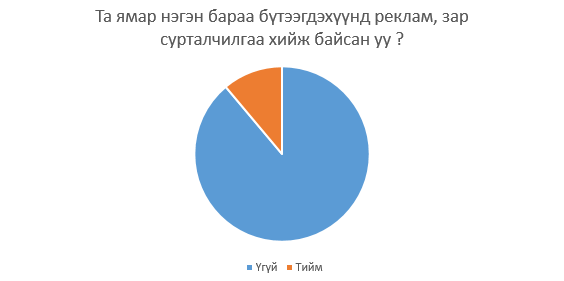
\includegraphics[scale=0.7]{Chart/Chart1}
	\caption[Хэрэглэгчийн судалгаа]{Реклам сурталчилгаа хийж байсан бэ?(Асуулга.)}
	\label{fig:Chart1}
\end{figure}

\begin{figure}[htbp]
	\centering
	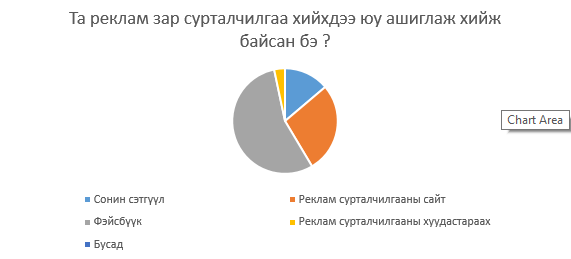
\includegraphics[scale=0.7]{Chart/Chart2}
	\caption[Хэрэглэгчийн судалгаа]{Реклам сурталчилгаа хийхдээ юу ашиглаж байсан бэ?(Асуулга.)}
	\label{fig:Chart2}
\end{figure}

\begin{figure}[htbp]
	\centering
	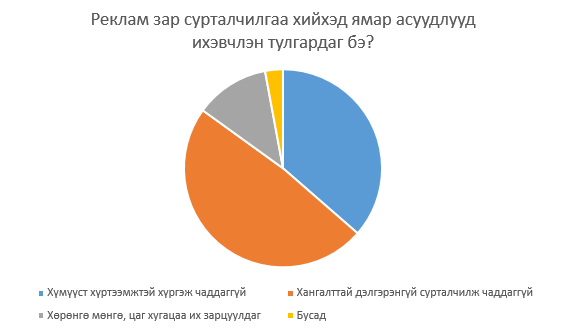
\includegraphics[scale=0.7]{Chart/Chart3}
	\caption[Хэрэглэгчийн судалгаа]{Тулгардаг асуудлууд(Асуулга.)}
	\label{fig:Chart3}
\end{figure}

\begin{figure}[htbp]
	\centering
	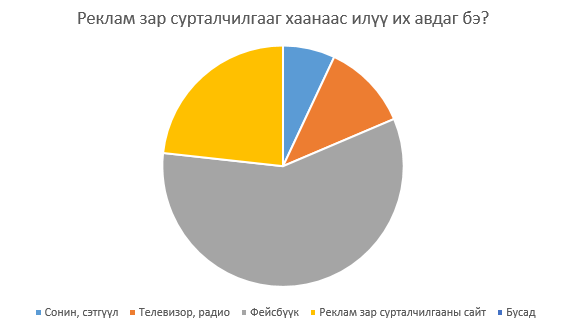
\includegraphics[scale=0.7]{Chart/Chart4}
	\caption[Хэрэглэгчийн судалгаа]{Реклам сурталчилгааг хаанаас авдаг бэ?(Асуулга.)}
	\label{fig:Chart4}
\end{figure}
\begin{figure}[htbp]
	\centering
	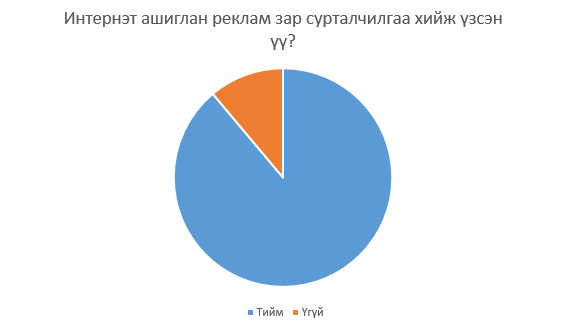
\includegraphics[scale=0.7]{Chart/Chart5}
	\caption[Хэрэглэгчийн судалгаа]{Интернэт ашиглан реклам хийж байсан уу?(Асуулга.)}
	\label{fig:Chart5}
\end{figure}

\begin{figure}[htbp]
	\centering
	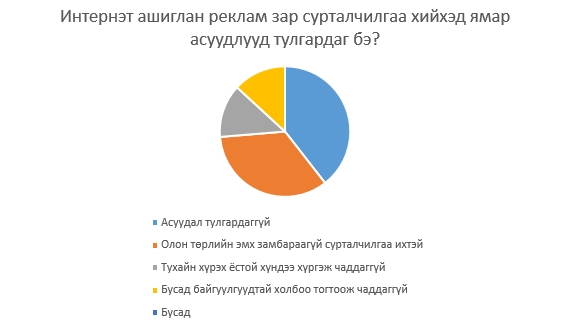
\includegraphics[scale=0.7]{Chart/Chart6}
	\caption[Интернэт ашиглан сурталчилгаа хийхэд тулгардаг асуудлууд]{Интернэт ашиглан сурталчилгаа хийхэд тулгардаг асуудлууд(Асуулга.)}
	\label{fig:Chart6}
\end{figure}

\begin{figure}[htbp]
	\centering
	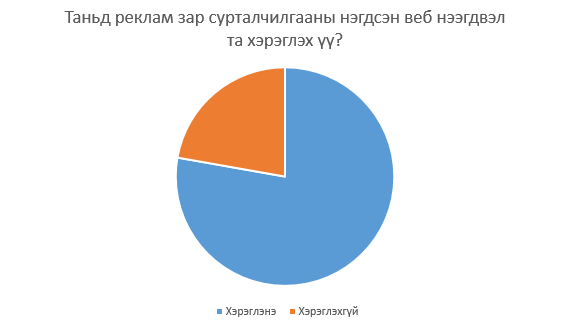
\includegraphics[scale=0.7]{Chart/Chart7}
	\caption[Хэрэглэгчийн судалгаа]{Сурталчилгааны веб нээгдвэл ашиглах эсэх(Асуулга.)}
	\label{fig:Chart7}
\end{figure}

%-------------------------------------------------------------------------------
\section{Хөгжүүлэлтэд ашиглах алгоритм}

\LaTeX{} бол Microsoft Word, Adobe Pages шиг \textsc{WYSIWYG} (Таны Харж байгаа Зүйл бол Таны Оруулсан Зүйл) төрлийн текст боловсруулах програм биш. \LaTeX{} --д зориулсан баримт нь үнэндээ \emph{хэвшүүлээгүй} задгай текст бүхий файл юм. Өөрийн тексттэй хамт түүнийг хэрхэн хэвшүүлэхийг тухай энгийн командыг бичиж, энэ файлаар \LaTeX{} --т хэлж өгдөг. Жишээ нь \emph{текстийг налуу болгож тодотгохдоо} \verb|\emph{text}| командыг ашиглах ба налуу болгох текстээ их хаалтанд бичнэ. Өөрөөр хэлбэл \LaTeX{} нь HTML -тэй маш төстэй ''{mark-up}'' хэл юм.

%-------------------------------------------------------------------------------

\section{Технологийн судалгаа}

\section{Laravel фреймворк}
Ларавел фреймворк нь  MVC вэб програмуудын хөгужилд зориулагдсан үнэгүй, нээлттэй эхтэй PHP вэб фреймворк юм. Ларавел нь MIT тусгай зөвшөөрөлтэй бөгөөд GitHub дээр байршдаг. PHP орчинд алдартай 2013 оны 12 сарын судалгаагаар Laravel  2014 оны хувьд хамгийн ирээдүйтэй PHP вэб фреймворк гэж судлагдсан байдаг.
PHP фреймворкүүдийг 2015 оны эцсийн байдлаар харьцуулж үзэхэд  хамгийн их хэрэглэгддэг фреймворк гэдэг нь судалгаагаар тогтоогдсон.

\section{MySQL}
MySQL нь холбоост өгөгдлийн санг удирдах систем юм. MySQL хэмээх нэрний хувьд уг системийг санаачлан хөгжүүлэгч Micheal Widenius-ын охины нэр My + SQL(Structed Query Language) гэсэн утгатай ажээ.
Энэ систем нь GNU (General Public License) буюу нээлтэй эхийн систем учир хүссэн хэн бүхэн хөгжүүлэлтэнд оролцож, үнэгүй хэрэглэж болох юм. Эзэмшигч нь алдарт Java-г хөгжүүлсэн Sun MicroSystems компани байсан ба, одоогоор Sun-г Oracle корпораци эзэмших болсон билээ.
Үнэгүй програм хангамжийн өгөгдлийн санг удирдах системд ихэвчлэн MySQL-ийг хэрэглэдэг бөгөөд тэдгээрийн сонгодог жишээ гэвэл Joomla, Drupal, Wordpress, phpBB гэх мэт агуулга удирдах системүүд (CMS-Content Management System), Wikipedia, Facebook, Google гэх мэт томоохон компаниуд хэрэглэдэг юм.
Хөгжүүлэлт нь C/C++ хэл дээр хийгдсэн ба AIX, BSDi, FreeBSD, HP-UX, i5/OS, Linux, Mac OS X, NetBSD, Novell NetWare, OpenBSD, OpenSolaris, eComStation, OS/2 Warp, QNX, IRIX, Solaris, Symbian, SunOS, SCO OpenServer, SCO UnixWare, Sanos, Tru64, Microsoft Windows гэсэн олон үйлдлийн системүүд дээр ажилладаг.
MySQL бол хамгийн өргөн хэрэглээтэй нээлттэй эхийн (Open Source) өгөгдлийн сан удирдах програм юм. Анх 1995 онд зах зээлд гарсан ба с/с++ хэл дээр бичигдсэн. Одоогийн байдлаар 5.7 нь хамгийн сүүлийн хувилбар болон гараад байна. Энэ сүүлийн хувилбар дээр нэмэгдсэн давуу талууд гэвэл 3 дахин хурдан үйл ажиллагаатай болсон мөн натив JSON дэмжигчтэй болсон гэх мэт шинэлэг үйлдлүүд нэмэгдсэн байна.

\section{Php}
  Rasmus Lerdorf WWW-д вэб хуудас үүсгэх үедээ өгөгдөл боловсруулах хялбархан арга хайж байгаад 1995 онд PHP хэлийг скрипт хэл байдлаар зохиосон.
PHP нь сервер талын скрипт хэл ба динамик вэб хуудас хийхэд илүү тохиромжтой. Энэ скрипт хэл нь энгийн хэрэглээний вэб сайтаас эхлээд байгууллагын иж бүрэн вэб программ хийж болохоор MySQL мэтийн өгөгдлийн сантай харилцан ажиллах боломжтой.
Хуудас ачаалах үед броузерээр нэг бүрчлэн уншдаг HTML-тэй адилгүй, PHP баримтыг бэлтгэхдээ серверээр урьдчилан боловсруулдаг. PHP код агуулсан хуудас нь хэрэглэгчийн броузерт илгээгдхээс өмнө серверээр боловсруулагдсан байдаг.
PHP хэлний өөр нэг давуу тал бол скриптэн хэл юм. Ихэнх програмчлалын хэлнүүдэд ажиллахын өмнө машины хэл рүү хөрвүүлэх тусгай файлууд /compile/ шаардлагатай байдаг бол PHP хэлний хувьд хөрвүүлэлт хийх шаардлагагүй байдаг тул код засварлах болон шалгахад илүү хурдан байдаг

\section{JQuery}
2006 оны эхээр АНУ-ын Нью-Иорк хотын BarCamp-д John Resig хэмээх вэб хөгжүүлэгч залуу jQuery сангийн тухай анх мэдэгджээ. Resig өөрийн вэб сайтдаа: Тухайн үед байгаа сангуудад сэтгэл дундуур байгаагаа, мөн түүнчлэн JavaScript – ий тухай бичилтийг нь багасгаснаар маш их ажил хөнгөвчлөх боломжтой, энгийн үйлдлүүдэд зориулан тусгай хэрэгслүүд нэмэх хэрэгтэй гэж дурдсан байдаг.
Хөгжүүлэх нийгэмлэгт jQuery нь томоохон амжилт авчирсан төдийгүй улмаар маш хурдтай хөгжсөн. Бусад хөгжүүлэгчид сан боловсронгуй болгоход тусалж эхэлснээр jQuery – гийн анхны хувилбар 1.0 нь 2006 оны 8-р сарын 26- нд гарсан.
Түүнээс хойш jQuery 3.1.1 хувилбар гарсан ба хөгжүүлэлтийн нийгэмлэгээс plug-in –ийг маш ихээр оруулсан. Plug-in нь jQuery – ийн сангийн цөм хэсэг биш харин нэмэлт хэрэгсэл юм. 
jQuery – гийн давуу талууд нь:
\begin{itemize}
\item Файлын хэмжээ бага
\item Маш энгийн бичилттэй
\item Холбоо бүхий method – уудтай
\item Санг өргөтгөх plug-in нь энгийн бүтэцтэй
\item Асар том онлайн нийгэмлэгтэй
\item JQueryUI мэтийн jQuery – гийн нэмэлт сонголтуудтай
\end{itemize}
\section{Service}
2006 оны эхээр АНУ-ын Нью-Иорк хотын BarCamp-д John Resig хэмээх вэб хөгжүүлэгч залуу jQuery сангийн тухай анх мэдэгджээ. Resig өөрийн вэб сайтдаа: Тухайн үед байгаа сангуудад сэтгэл дундуур байгаагаа, мөн түүнчлэн JavaScript – ий тухай бичилтийг нь багасгаснаар маш их ажил хөнгөвчлөх боломжтой, энгийн үйлдлүүдэд зориулан тусгай хэрэгслүүд нэмэх хэрэгтэй гэж дурдсан байдаг.
Хөгжүүлэх нийгэмлэгт jQuery нь томоохон амжилт авчирсан төдийгүй улмаар маш хурдтай хөгжсөн. Бусад хөгжүүлэгчид сан боловсронгуй болгоход тусалж эхэлснээр jQuery – гийн анхны хувилбар 1.0 нь 2006 оны 8-р сарын 26- нд гарсан.
Түүнээс хойш jQuery 3.1.1 хувилбар гарсан ба хөгжүүлэлтийн нийгэмлэгээс plug-in –ийг маш ихээр оруулсан. Plug-in нь jQuery – ийн сангийн цөм хэсэг биш харин нэмэлт хэрэгсэл юм. 
jQuery – гийн давуу талууд нь:
\begin{itemize}
\item Файлын хэмжээ бага
\item Маш энгийн бичилттэй
\item Холбоо бүхий method – уудтай
\item Санг өргөтгөх plug-in нь энгийн бүтэцтэй
\item Асар том онлайн нийгэмлэгтэй
\item JQueryUI мэтийн jQuery – гийн нэмэлт сонголтуудтай
\end{itemize}
\section{Бүлгийн дүгнэлт}
%-------------------------------------------------------------------------------
% Бүлэг 2

\book{Бизнес эрхлэгчдийн сурталчилгааны нэгдсэн вебийн судалгаа} % Бүлгийн нэр
\label{Chapter2} % Энэ бүлэг рүү ишлэл хийх бол \ref{Chapter1} командыг ашигла 

\section{Системийн үйл ажиллагааны тухай дэлгэрэнгүй }
Энэхүү систем нь реклам зар сурталчилгааг явуулах шаардлагатай үйлдвэрлэл, үйл ажиллагаагаа явуулдаг хувь хүн болоод албан байгуулага, худалдааны гэх мэт бүхий л газрууд өөрт тохируулан ашиглах боломжтой. Реклам зар сурталчилгаа хийхээс гадна хүмүүсийн санал бодлыг хүлээн авах, хариу өгөх зөвлөх зэрэг үйл ажиллагаа байхаас гадна арга хэмжээ, урамшуулалын мэдээллийг хүмүүст хүргэх боломжтой юм.

\section{Системийг ашиглах хэрэглэгчид}
Реклам зар сурталчилгааг нийтэд хүргэх шаардлагатай нийгмийн бүхий л аж ахуйн нэгжүүдэд хэрэглэгдэх боломжтой юм.
Жишээ нь: 
\begin{itemize}
\item Хувиараа бизнес эрхлэгчид
\item Бараа бүтээгдэхүүн үйлдвэрлэгчид
\item Худалдаа наймаачид	
\item Үйл ажиллагаа явуулдаг албан байгуулгууд
\item Хувийн байгуулагууд
\item олон нийтийн байгуулагууд
\item Хувь хүн
\end{itemize}
\section{Функционал шаардлага}
 Энэхүү веб нь хэрэглэгч, админ,зочин гэсэн 3-н оролцогчтой.
Хэрэглэгч нь: Өөрийн үйлдэрлэлийн чиглэлээр хуудас үүсгэн сурталчилах, бусдад түгээх боломжтой.
Админ: Бүх хуудсыг хянах, бүртгэлтэй хэрэглэгч болон вебийн ерөнхий мэдээллийг удирдах.
Зочин:Хуудаснуудын мэдээллийг харах,сэтгэгдэл бичих,үнэлгээ өгөх ба шаардлагатай тохиолдолд бүргүүлэх боломжтой.
Хэрэглэгчийн функциональ шаардлага:
\begin{enumerate}
	\item Өөрийн үйлдвэрлэлийн чиглэлээр вебд хуудас үүсгэх
	\item Хуудсандаа бараа, бүтээгдэхүүний танилцуулага удирдах
	\begin{enumerate}
		\item[2.1] Танилцуулага нэмэх
		\item[2.2] Танилцуулага хасах
		\item[2.3] Өөрчлөх
	\end{enumerate}
	\item Зочидын сэтгэгдэлд хариу бичих
	\item Арга хэмжээ зарлах
\end{enumerate}
Админы функциональ шаардлага:
\begin{enumerate}
	\item Тайлан гаргах
	\begin{enumerate}
		\item[1.1] Вебд хандсан зочидын тайлан
		\item[1.2] Дэлгүүрийн тайлан
	\end{enumerate}
	\item Вебийн бүх хуудсийг удирдах
	\begin{enumerate}
		\item[2.1] Хуудас устгах
		\item[2.2] Хуудсанд сануулга өгөх
	\end{enumerate}
	\item Вебийн ерөнхий реклам зар сурталчилгааг удирдах
	\begin{enumerate}
		\item[3.1] Реклам зар сурталчилгааг устгах
		\item[3.2] Реклам зар сурталчилгааг нэмэх
		\item[3.3] Реклам зар сурталчилгааг өөрчлөх
	\end{enumerate}
\end{enumerate}
Зочины функциональ шаардлага
\begin{enumerate}
	\item Реклам зар сурталчилгаа харах
	\item Реклам зар сурталчилгаанд сэтгэгдэл үлдээх
	\begin{enumerate}
		\item[2.1] Вебд бүртгүүлэх
	\end{enumerate}	
	
	\item Реклам зар сурталгаанд үнэлгээ өгөх
	\begin{enumerate}
		\item[3.1] Вебд бүртгүүлэх
	\end{enumerate}	
	
	\item Арга хэмжээнд санал өгөх
	\item Вебээс хайлт хийх
	\begin{enumerate}
		\item[5.1] Хуудас хайх
		\item[5.2] Арга хэмжээ хайх
	\end{enumerate}
\end{enumerate}
\section{Функционал бус шаардлага}
\begin{enumerate}
	\item Өгөгдлийн сан ачааллах хугацаа нь хурдан шуурхай байх. Бүх өгөгдлүүд өгөгдлийн санд хадгалагдсан байх болно
	\item Вебд 1000-с 10000-хүн нэгэн зэрэг хандаж үйл ажиллагаа явуулах учир серверийн хүчин өндөр байх
	\item Архитектурын хувьд windows орчинд хөгжүүлэгдэнэ.Вебийн хөгжүүлэлт нь CodeIgniter framework – той хамтран ажиллаж боломжтой хэлүүд дээр хийгдэнэ.
	\item Кодчилолын хувьд CodeIgniter framework –ийн стандартын дагуу хийгдэнэ.
\end{enumerate}
\section{Юзкейс диаграм}
\begin{figure}[htbp]
	\centering
	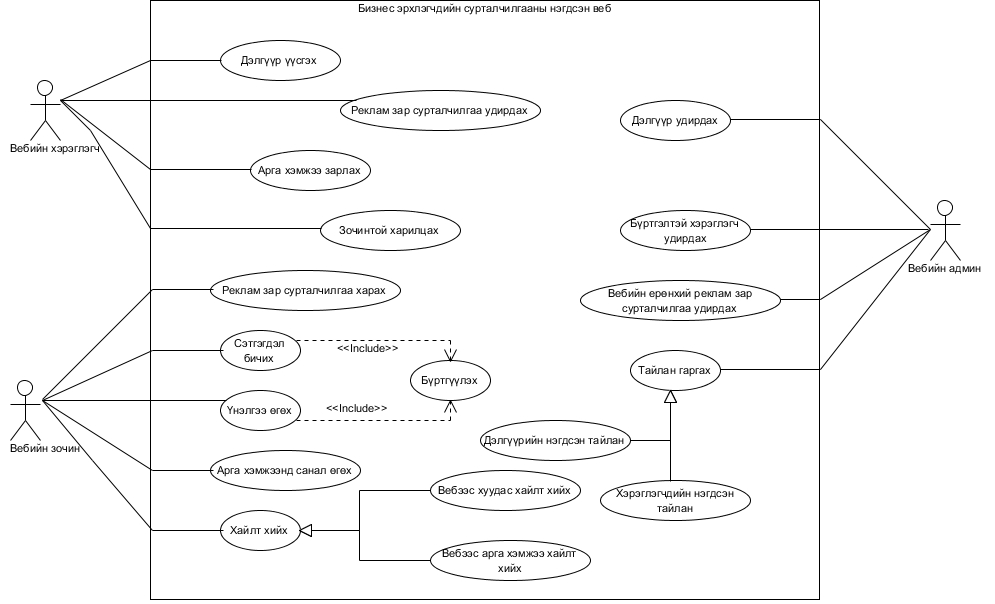
\includegraphics[scale=0.4]{Diagrams/UseCase}
	\caption[Юзкейс диаграм]{Юзкейс диаграм}
	\label{fit:UseCase}
\end{figure}
\section{Юзкейс диаграмын тодорхойлолт}

\begin{center}
	\begin{table}[!htbp]
		\caption{}
		\begin{tabular}{|p{4cm}|p{11cm}|}
		\hline
			Нэр: & Дэлгүүр үүсгэх \\
		\hline
			ID: & 1 \\
		\hline
			Товч тайлбар: & Хэрэглэгч нь веб серверд шинээр бүртгэл үүсгэнэ. \\
		\hline
			Триггер: & Хэрэглэгч нь бүртгүүлэх шаардлагатай болсон. \\
		\hline
			Үндсэн оролцогч: & Хэрэглэгч \\
		\hline
			Хоёрдогч оролцогч: & Байхгүй  \\
		\hline
			Өмнөх нөхцөл: &  Веб сервер ажиллагаатай байх\\
		\hline
			Ажлын урсгал: & \begin{enumerate}
						 	\item Суралцагч нь бүртгүүлэхийг сонгосноор энэ юз кейс эхлэнэ. 
						 	\item Веб сервер нь суралцагчид бүртгүүлэх цонхыг харуулна. 
						 	\item Хэрэглэгч нь өөрийн мэдээллийг (өөрийн нэр, имэйл хаяг, нууц үгээ) оруулна. 
						 	\item Веб сервер нь хэрэглэгчийн оруулсан мэдээллийг шалгана. 
						 	\item IF (“мэдээлэл үнэн зөв бол”)
							 	\begin{enumerate}
							 		\item[5.1] Веб сервер хэрэглэгчийн оруулсан мэдээллийг (өөрийн нэр, имэйл хаяг, нууц үгээ) баазад хадгална.
							 		\item[5.2] Веб сервер хэрэглэгчийг амжилттай бүртгүүлсэнийг нь харуулна. 
							 	\end{enumerate}
						 	\item ELSE
							 	\begin{enumerate}
							 		\item[6.1] Веб сервер нь хэрэглэгчийн оруулсан мэдээлэл бүрийг шалгана.  
							 		\item[6.2] Веб сервер нь алдаатай оруулсан мэдээллийг тодруулж харуулна. 
							 		\item[6.3] Веб сервер нь мэдээллийг дахин оруулахыг асууна. 
							 	\end{enumerate}
						  \end{enumerate}
\\					  \hline
				Дараах нөхцөл: &
				 \begin{enumerate}
									\item Хэрэглэгч веб серверд бүртгэлтэй болсон байна. 
									\item Хэрэглэгчийн мэдээлэл баазад хадгалагдсан байна. 
				\end{enumerate}	   
\\				   \hline
				Альтернатив урсгал: &  \begin{enumerate}
									\item Хэрэглэгч бүртгэлийг цуцалсан.
									\item Веб сервер дээр алдаа гарсан. 
										\end{enumerate}
				\\	\hline
		\end{tabular}
	\end{table}
\end{center}


\begin{center}
	\begin{table}[!htbp]
		\caption{}
		\begin{tabular}{|p{4cm}|p{11cm}|}
			\hline
			Нэр: & Реклам зар сурталчилгаа удирдах \\
			\hline
			ID: & 2 \\
			\hline
			Товч тайлбар: & Хэрэглэгч веб серверд шинээр реклам зар сурталчилгаа нэмнэ.  \\
			\hline
			Триггер: & Хэрэглэгч реклам зар сурталчилгаа нэмэхийг хүссэн. \\
			\hline
			Үндсэн оролцогч: & Хэрэглэгч \\
			\hline
			Хоёрдогч оролцогч: & Веб  \\
			\hline
			Өмнөх нөхцөл: &  \begin{enumerate}
								\item Хэрэглэгч өөрийн эрхээрээ нэвтэрсэн байх.
								\item Веб сервер ажиллагаатай байх.
							\end{enumerate}
\\			\hline
			Ажлын урсгал: & \begin{enumerate}
								\item Хэрэглэгч реклам зар сурталчилгаа нэмэхийг сонгосноор энэ юз кейс эхлэнэ.
								\item Веб нь реклам зар сурталчилгаа нэмэх хуудсыг хэрэглэгчид харуулна.
								\item Хэрэглэгч реклам зар сурталчилгааныхаа замыг зааж өгнө.
								\item Веб тухайн реклам зар сурталчилгаа мөн эсэхийг шалгана.
								\item IF (реклам зар сурталчилгаа байгаа бол)
									\begin{enumerate}
										\item[5.1] Веб тухайн реклам зар сурталчилгааг баазруу ачаална.
										\item[5.2] IF (амжилттай ачаалагдсан бол)
											\begin{enumerate}
												\item[5.2.1] Амжилттай ачаалагдсан мэдээллийг хэрэглэгчид харуулна.
											\end{enumerate}
										\item[5.3] Else
											\begin{enumerate}
												\item[5.3.1] Веб ачаалах үеийн алдааг хэрэглэгчид харуулна.
											\end{enumerate}
										\item[5.4] Веб зөв зам дахин оруулахыг асууна.
								\end{enumerate}
							\end{enumerate}
\\						\hline
			Дараах нөхцөл: &  Вебд реклам зар сурталчилгаа байршисан байна. \\
			\hline
			Альтернатив урсгал: &  Вебийн өгөгдлийн сангын багтаамж дүүрсэн. \\
			\hline
		\end{tabular}
	\end{table}
\end{center}

\begin{center}
	\begin{table}[!htbp]
		\caption{}
		\begin{tabular}{|p{4cm}|p{11cm}|}
			\hline
			Нэр: & Арга хэмжээ зарлах \\
			\hline
			ID: & 3 \\
			\hline
			Товч тайлбар: & Хэрэглэгч өөрийн хуудсаар дамжуулан удахгүй болох арга хэмжээг зарлана.  \\
			\hline
			Триггер: & Хэрэглэгч арга хэмжээ зарлахыг хүссэн. \\
			\hline
			Үндсэн оролцогч: & Хэрэглэгч \\
			\hline
			Хоёрдогч оролцогч: & Байхгүй  \\
			\hline
			Өмнөх нөхцөл: &  \begin{enumerate}
				\item Вебд  өөрийн хуудсаа нээсэн байх.
				\item Веб хэвийн ажиллагаатай байх.
			\end{enumerate}
			\\			\hline
			Ажлын урсгал: & \begin{enumerate}
								\item Хэрэглэгч арга хэмжээ зарлах хэсгийг сонгосоноор энэхүү энэ юзкейс эхэлнэ.
								\item Веб арга хэмжээний тухай бөглөх хуудсыг харуулна
								\item Хэрэглэгч хуудсийг (арга хэмжээ эхлэх, дуусах огноо, тайлбар ) бөглөнө.
								\item IF( Мэдээлэл үнэн бөглөсөн бол )
									\begin{enumerate}
										\item[4.1] Веб арга хэмжээ баталгаажуулах хэсгийг харуулна
									\end{enumerate}
								\item ELSE 
									\begin{enumerate}
										\item[5.1] Веб хэрэглэгчийн оруулсан мэдээлэл алдаатайг мэдэгдэнэ.
										\item[5.2] Хэрэглэгч хуудсыг дахин бөглөнө.
									\end{enumerate}
								\item Хэрэглэгч арга хэмжээг баталгаажуулах хэсгийг сонгоно.
								\item Веб арга хэмжээ амжилттай баталгаажсаныг мэдэгдэнэ.
							\end{enumerate}
\\						\hline
			Дараах нөхцөл: & Арга хэмжээ зарлагдсан байна. \\
			\hline
			Альтернатив урсгал: & Хэрэглэгч арга хэмжээг цуцалсан байна. \\
			\hline
		\end{tabular}
	\end{table}
\end{center}


\begin{center}
	\begin{table}[!htbp]
		\caption{}
		\begin{tabular}{|p{4cm}|p{11cm}|}
			\hline
			Нэр: & Зочинтой харилцах \\
			\hline
			ID: & 4 \\
			\hline
			Товч тайлбар: & Хуудасанд үлдээсэн зочины сэтгэгдэлд хариу бичих.  \\
			\hline
			Үндсэн оролцогч: & Хэрэглэгч \\
			\hline
			Хоёрдогч оролцогч: & Зочин  \\
			\hline
			Өмнөх нөхцөл: &  \begin{enumerate}
				\item Өөрийн хуудсанд нэвтэрсэн байх.
				\item Сэтгэгдэл үлдээсэн зочин вебд бүртгэлтэй байх.
			\end{enumerate}
			\\			\hline
			Ажлын урсгал: & \begin{enumerate}
								\item Хэрэглэгч зочины үлдээсэн сэтгэгдэлд хариу бичих хэсгийг сонгосоноор энэ юзкейс эхэлнэ.
								\item Веб хариу бичих талбарыг нээж харуулна.
								\item Хэрэглэгч зочины сэтгэгдэлд хариу бичнэ.
								\item Хэрэглэгч хариу сэтгэгдэлээ илгээнэ.
								\item Веб хариу сэтгэгдэл амжилттай илгээгдсэнийг мэдэгдэнэ.
							\end{enumerate} \\
						\hline
			Дараах нөхцөл: & Хэрэглэгч зочины сэтгэгдэлд хариу бичсэн байна. \\
			\hline
			Альтернатив урсгал: & Хэрэглэгч бичсэн сэтгэгдэлээ устгасан байна. \\
			\hline
		\end{tabular}
	\end{table}
\end{center}

\begin{center}
	\begin{table}[!htbp]
		\caption{}
		\begin{tabular}{|p{4cm}|p{11cm}|}
			\hline
			Нэр: & Реклам зар сурталчилгаа харах  \\
			\hline
			ID: & 5 \\
			\hline
			Товч тайлбар: & Зочин вебийн реклам зар сурталчилгааг харна.  \\
			\hline
			Үндсэн оролцогч: & Зочин \\
			\hline
			Хоёрдогч оролцогч: & Байхгүй  \\
			\hline
			Өмнөх нөхцөл: &  Вебд нэвтэрсэн байх \\
			\hline
			Ажлын урсгал: &  \begin{enumerate}
								\item Зочин вебд реклам зар сурталчилгаа харах зорилготой нэвтэрсэнээр энэ юзкейс эхэлнэ.
								\item Веб реклам зар сурталчилгааны төрлүүдийг харуулна. 
								\item Зочин реклам зар сурталчилгааныхаа төрлөө сонгоно сонгоно.
								\item Веб зочины сонгосон төрлийг харуулна.  
							\end{enumerate}	 \\
						\hline
			Дараах нөхцөл: & Зочин реклам зар сурталчилгаа харсан байна \\
			\hline 
			Альтернатив урсгал: & Байхгүй \\
			\hline
		\end{tabular}
	\end{table}
\end{center}

\begin{center}
	\begin{table}[!htbp]
		\caption{} 
		\begin{tabular}{|p{4cm}|p{11cm}|}
			\hline
			Нэр: & Сэтгэгдэл бичих  \\
			\hline
			ID: & 6 \\
			\hline
			Товч тайлбар: & Зочин хуудсанд сэтгэгдэл үлдээх.  \\
			\hline
			Үндсэн оролцогч: & Зочин \\
			\hline
			Хоёрдогч оролцогч: & Байхгүй  \\
			\hline
			Өмнөх нөхцөл: &  Вебд бүртгэлтэй байх \\
			\hline
			Ажлын урсгал: & \begin{enumerate}
								\item Зочин сэтгэгдэл үлдээх хэсгийг сонгосоноор энэ юзкейс эхэлнэ
								\item Веб зочинд сэтгэгдэл үлдээх хэсгийг харуулна
								\item Зочин хэсгийг сонгоно
								\item IF( Зочин вебд бүртгэлгүй бол )
									\begin{enumerate}
										\item[4.1] Веб бүртгэлийн хуудсийг харуулна
									\end{enumerate}
								\item ELSE
									\begin{enumerate}
										\item[5.1] Зочин сэтгэгдэл үлдээх хэсэгт сэтгэгдэлээ үлдээнэ
									\end{enumerate}
								\item Зочин сэтгэгдэл баталгаажуулах хэсгийг сонгоно
								\item Веб сэтгэгдэл амжилттай үлдээснийг мэдэгдэнэ.
							\end{enumerate} 	
\\				\hline
			Дараах нөхцөл: & Зочин хуудсанд сэтгэгдэл үлдээсэн байна. \\
			\hline
			Альтернатив урсгал: & Зочин сэтгэгдэлээ устгасан байна. \\
			\hline
		\end{tabular}
	\end{table}
\end{center}

\begin{center}
	\begin{table}[!htbp]
		\caption{} 
		\begin{tabular}{|p{4cm}|p{11cm}|}
			\hline
			Нэр: & Хайлт хийх  \\
			\hline
			ID: & 7 \\
			\hline
			Товч тайлбар: & Зочин вебээс өөрийн хүссэн реклам зар сурталчилгааг хайна.  \\
			\hline
			Үндсэн оролцогч: & Зочин \\
			\hline
			Хоёрдогч оролцогч: & Байхгүй  \\
			\hline
			Өмнөх нөхцөл: &  Вебд нэвтэрсэн байх \\
			\hline
			Ажлын урсгал: & \begin{enumerate}
								\item Зочин хайлт хийх хэсгийг сонгосоноор энэхүү юзкейс эхэлнэ
								\item Веб хайлт хийх төрлүүдийг харуулна харуулна
								\item Зочин хайлт хийх төрөлөө сонгоно
								\item Веб зочины сонгосон хайлт хийх хэсгийг харуулна
								\item Зочин хайлтын утгаа оруулна
								\item IF(Хайлтын утга алдаатай бол)
									\begin{enumerate}
										\item[6.1] Веб хайлтын утга алдаатайг зочинд мэдэгдэнэ.
										\item[6.2] Веб зочинд зөв хайлтын жишээ утга харуулна
									\end{enumerate}	
								\item ELSE IF(Таны хайсан утга )
									\begin{enumerate}
										\item[7.1] Веб таны хайсан утга илэрцгүй 
									\end{enumerate}
								\item Зочин хайлтанд илэрсэн утгуудыг харуулна
							\end{enumerate} 	\\
						\hline
			Дараах нөхцөл: & Зочин вебээс хүссэн хайлтаа олсон байна. \\
			\hline
			Альтернатив урсгал: & Зочины хайлт илэрцгүй байна.\\
			\hline
		\end{tabular}
	\end{table}
\end{center}

\begin{center}
\begin{table}[!htbp]
	\caption{}
	\begin{tabular}{|p{4cm}|p{11cm}|}
		\hline
		Нэр: & Арга хэмжээнд санал өгөх  \\
		\hline
		ID: & 8 \\
		\hline
		Товч тайлбар: & Зочин хуудсануудын арга хэмжээнд санал өгөх боломжтой.  \\
		\hline
		Үндсэн оролцогч: & Зочин \\
		\hline
		Хоёрдогч оролцогч: & Байхгүй  \\
		\hline
		Өмнөх нөхцөл: &  Зочин вебд бүртгэлтэй байх. \\
		\hline
		Ажлын урсгал: & \begin{enumerate}
							\item Зочин арга хэмжээнд санал өгөх хэсгийг сонгосоноор энэ юзкейс эхэлнэ.
							\item Веб арга хэмжээнд санал өгөх хэсгийг харуулна
							\item Зочин санал өгөх хэсгийг сонгоно.
							\item IF( Зочин вебд бүртгэлгүй бол )
								\begin{enumerate}
									\item[4.1] Веб бүртгэлийн хуудсийг харуулна
								\end{enumerate}
							\item ELSE
								\begin{enumerate}
									\item[5.1] Зочин арга хэмжээнд санал өгнө
								\end{enumerate}
							\item Зочин санал баталгаажсаны веб мэдэгдэнэ
						\end{enumerate}	\\
		\hline
		Дараах нөхцөл: & Зочин арга хэмжээнд санал өгсөн байна. \\
		\hline
		Альтернатив урсгал: & Зочин саналаа устгасан байна. \\
		\hline
	\end{tabular}
\end{table}
\end{center}

\begin{center}
	\begin{table}[!htbp]
		\caption{}
		\begin{tabular}{|p{4cm}|p{11cm}|}
			\hline
			Нэр: & Бүртгэлтэй хэрэглэгч удирдах  \\
			\hline
			ID: & 9 \\
			\hline
			Товч тайлбар: & Админ бүртгэлтэй зочиныг вебээс хасах.  \\
			\hline
			Үндсэн оролцогч: & Админ \\
			\hline
			Хоёрдогч оролцогч: & Байхгүй  \\
			\hline
			Өмнөх нөхцөл: &  Зочин вебд зүй зохисгүй зүйл хийх. \\
			\hline
			Ажлын урсгал: & \begin{enumerate}
								\item Админ бүртгэлтэй зочидын жагсаалтыг сонгосоноор энэ юзкейс эхэлнэ.
								\item Веб бүртгэлтэй зочидын жагсаалтыг харуулна
								\item Админ зөрчилтэй зочинг сонгоно
								\item Веб зөрчилтэй зочины мэдээллийг харуулна
								\item Админ зөрчилтэй зочинг вебээс хасна
								\item Веб зөрчилтэй зочин амжилттэй вебээс хасагдсаныг мэдэгдэнэ.
							\end{enumerate}	\\
						\hline
			Дараах нөхцөл: & Зөрчилтэй зочин вебээс хасагдсан байна.(Бүртгэлтэй зочидын сангаас хасагдах ) \\
			\hline
			Альтернатив урсгал: & Админ зочинг буцаан сэргээсэн байна. \\
			\hline
		\end{tabular}
	\end{table}
\end{center}

\begin{center}
	\begin{table}[!htbp]
		\caption{}
		\begin{tabular}{|p{4cm}|p{11cm}|}
			\hline
			Нэр: & Сайтын ерөнхий реклам зар сурталчилгааг удирдах  \\
			\hline
			ID: & 10 \\
			\hline
			Товч тайлбар: & Сайтын ерөнхий реклам зар сурталчилгааг нэмэх, хасах, өөрчлөх боломжтой.  \\
			\hline
			Үндсэн оролцогч: & Админ \\
			\hline
			Хоёрдогч оролцогч: & Байхгүй  \\
			\hline
			Өмнөх нөхцөл: &  Админ эрхээр нэвтэрсэн байх. \\
			\hline
			Ажлын урсгал: & \begin{enumerate}
								\item Админ сайтын ерөнхий реклам зар сурталчилгаа удирдах хэсгийг сонгосоноор энэ юзкейс эхэлнэ
								\item Веб реклам зар сурталчилгаа удирдах төрлүүдийг харуулна
								\item Админ реклам зар сурталчилгаа нэмэх хэсгийг сонгоно
								\item Веб нь реклам зар сурталчилгаа нэмэх хуудсыг админд харуулна.
								\item Админ реклам зар сурталчилгааныхаа замыг зааж өгнө.
								\item Веб тухайн реклам зар сурталчилгаа мөн эсэхийг шалгана.
								\item IF (реклам зар сурталчилгаа байгаа бол)
									\begin{enumerate}
										\item[7.1] Веб тухайн реклам зар сурталчилгааг баазруу ачаална.
										\item[7.2] IF (амжилттай ачаалагдсан бол)
											\begin{enumerate}
												\item[7.2.1] Амжилттай ачаалагдсан мэдээллийг админд харуулна. 
											\end{enumerate}
										\item[7.3] Else
											\begin{enumerate}
												\item[7.3.1] Веб ачаалах үеийн алдааг админд харуулна. 
											\end{enumerate}
										\item[7.4] Веб зөв зам дахин оруулахыг асууна.
									\end{enumerate}
								\item Вебийн ерөнхий реклам зар сурталчилгаа амжилттай нэмэгдсэнийг мэдэгдэнэ.
						\end{enumerate}	\\
					\hline
			Дараах нөхцөл: & Вебийн ерөнхий реклам зар сурталчилгаа нэмэгдсэн байна \\
			\hline
			Альтернатив урсгал: & Админ буцааж устгасан байна \\
			\hline
		\end{tabular}
	\end{table}
\end{center}
%-------------------------------------------------------------------------------
\section{Шинжилгээний класс диаграм}

\begin{figure}[!h]
	\centering
	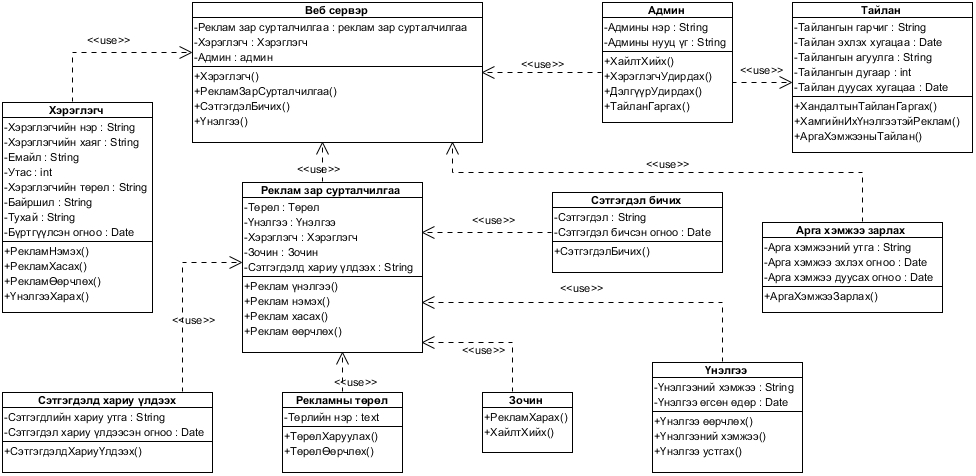
\includegraphics[angle=90,scale=0.7]{Diagrams/SClass}
	\caption[Шинжилгээний класс диаграм]{Шинжилгээний класс диаграм}
	\label{fig:SClass}
\end{figure}

%--------------------------------------------------------------
\section{Шинжилгээний дарааллын диаграм}
\begin{figure}
	\centering
	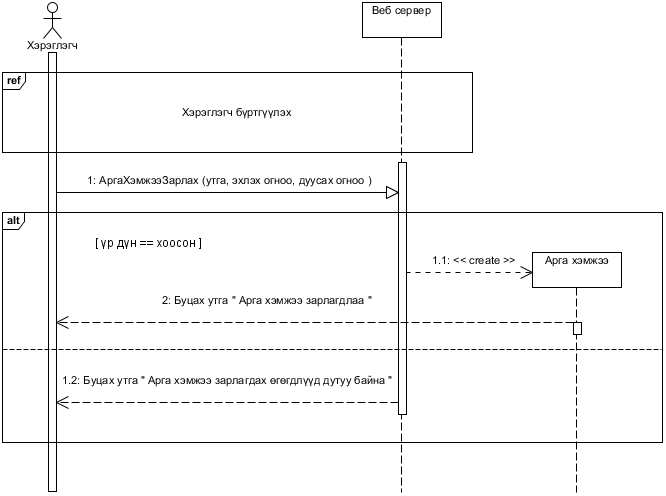
\includegraphics[scale=0.7]{Diagrams/arga_hemjee}
	\caption[Арга хэмжээ зарлах шинжилгээний дарааллын диаграм]{Арга хэмжээ зарлах шинжилгээний дарааллын диаграм}
	\label{text}
\end{figure}

\begin{figure}
	\centering
	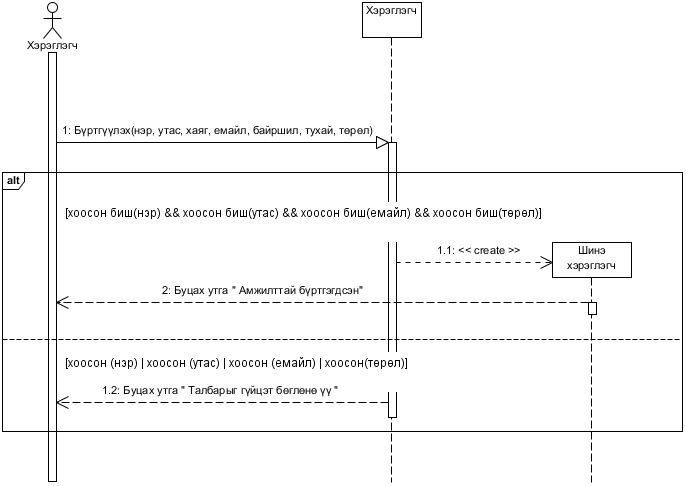
\includegraphics[scale=0.65]{Diagrams/create}
	\caption[Бүртгүүлэх шинжилгээний дарааллын диаграм]{Бүртгүүлэх шинжилгээний дарааллын диаграм}
	\label{text}
\end{figure}

\begin{figure}
	\centering
	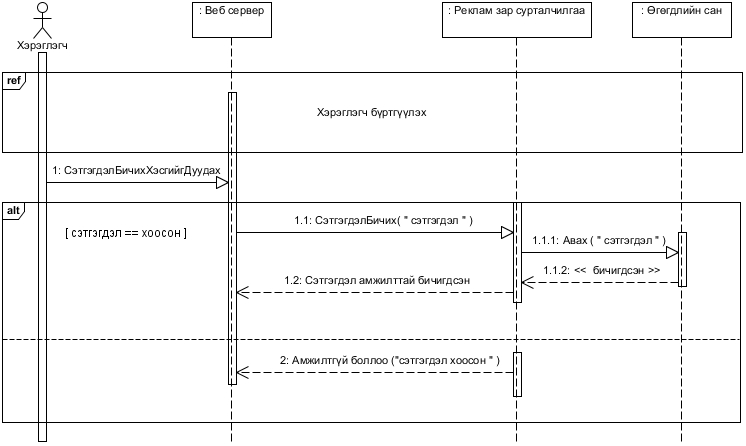
\includegraphics[scale=0.6]{Diagrams/write}
	\caption[Сэтгэгдэл бичих шинжилгээний дарааллын диаграм]{Сэтгэгдэл бичих шинжилгээний дарааллын диаграм}
	\label{text}
\end{figure}

\section{Үйл ажиллагааны диаграм}
\begin{figure}
	\centering
	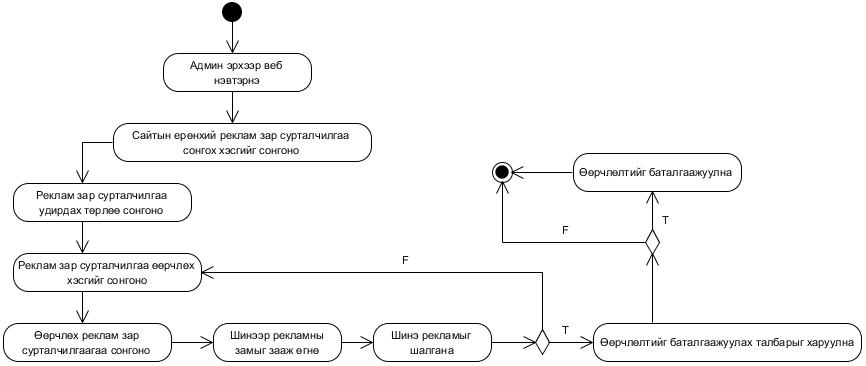
\includegraphics[scale=0.5]{Diagrams/change}
	\caption[Сайтын ерөнхий реклам удирдах үйл ажиллагааны диаграм]{Сайтын ерөнхий реклам удирдах үйл ажиллагааны диаграм}
	\label{text}
\end{figure}
\begin{figure}
	\centering
	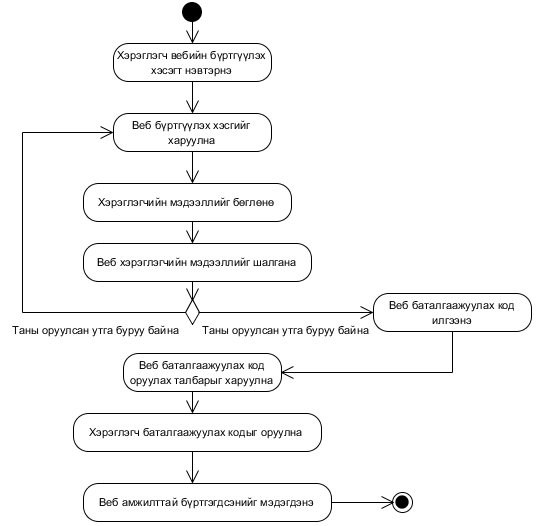
\includegraphics[scale=0.75]{Diagrams/sign_up}
	\caption[Бүртгүүлэх үйл ажиллагааны диаграм]{Бүртгүүлэх үйл ажиллагааны диаграм}
	\label{text}
\end{figure}
\begin{figure}
	\centering
	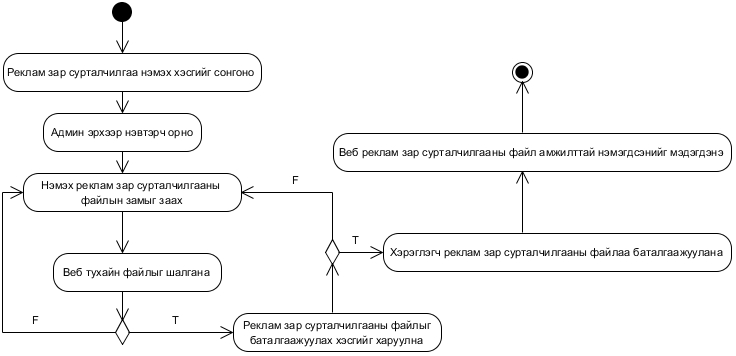
\includegraphics[scale=0.6]{Diagrams/add}
	\caption[Реклам зар сурталчилгаа нэмэх үйл ажиллагааны диаграм]{Реклам зар сурталчилгаа нэмэх үйл ажиллагааны диаграм}
	\label{text}
\end{figure}
\begin{figure}
	\centering
	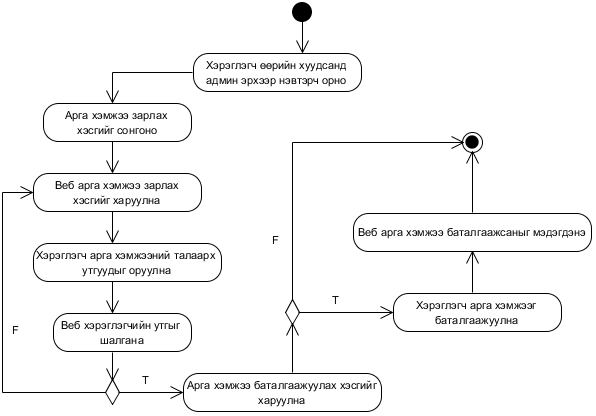
\includegraphics[scale=0.75]{Diagrams/event}
	\caption[Арга хэмжээ зарлах үйл ажиллагааны диаграм]{Арга хэмжээ зарлах үйл ажиллагааны диаграм}
	\label{text}
\end{figure}
\begin{figure}
	\centering
	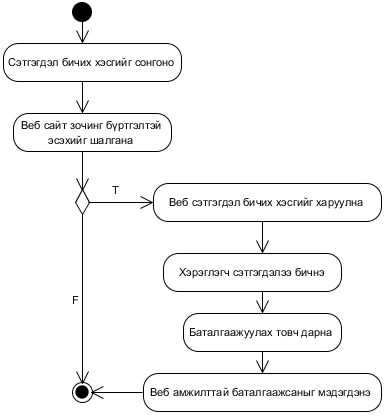
\includegraphics[scale=0.75]{Diagrams/comment}
	\caption[Сэтгэгдэл бичих үйл ажиллагааны диаграм]{Сэтгэгдэл бичих үйл ажиллагааны диаграм}
	\label{text}
\end{figure}w

\begin{figure}
	\centering
	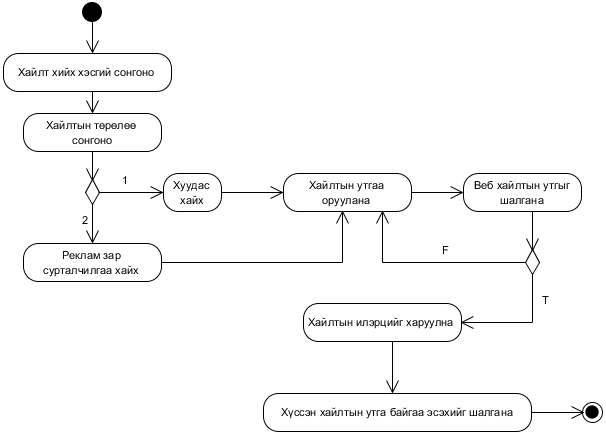
\includegraphics[scale=0.7]{Diagrams/search}
	\caption[Хайлт хийх үйл ажиллагааны диаграм]{Хайлт хийх үйл ажиллагааны диаграм}
	\label{text}
\end{figure}


\section{Бүлгийн дүгнэлт}
Хэрэглэгчийн шаардлагаа тодорхойлж тодорхойлсон шаардлага бүрээ нягтлан хянаж функционал болон фунционал бусаар нь ялгасан. Функционал шаардлага дээрээ үндэслэн юз кейс диаграмаа гаргасан ба бүх  юзкейс бүрт тодорхойлолт гаргасан. Мөн тодорхойлолт бичсэн юзкейс диаграм бүртээ үйл ажиллагааны диаграм зурсан үйл ажиллагааг нь илүү нарийн ойлгомжтой болгож өгч байна.

 
% Бүлэг 3

\chapter{Системийн зохиомж} % Зарим нэг зөвлөмж
\label{Chapter3} % Энэ бүлэг рүү ишлэл хийх бол \ref{Chapter2} командыг ашигла 

	\section{Өгөгдлийн ерөнхий схем}
		\begin{figure}[h!]
			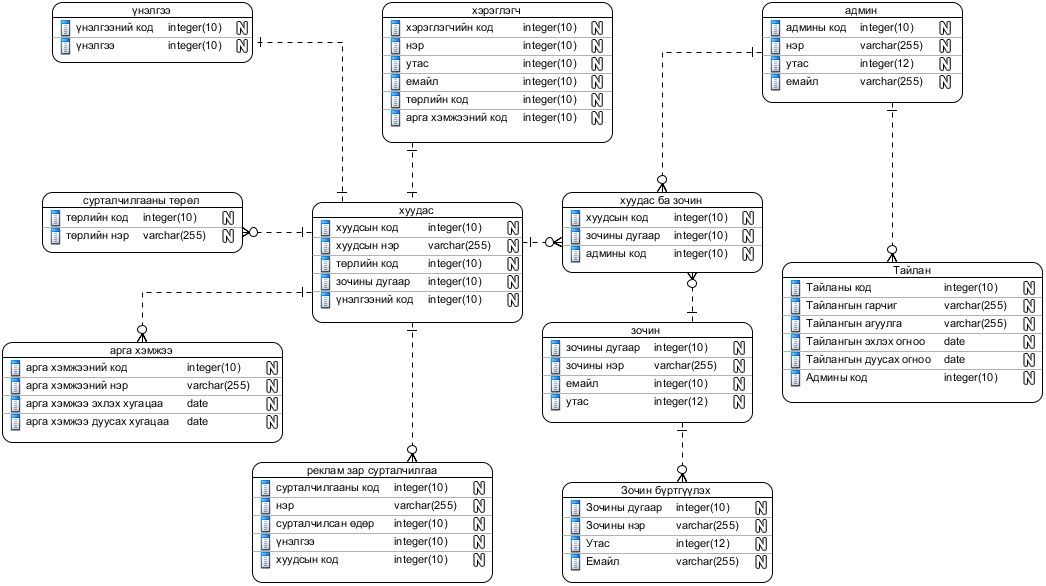
\includegraphics[width=27cm,angle=90,scale=0.7]{Diagrams/Entity}
			\caption[Өгөгдлийн ерөнхий схем]{Өгөгдлийн ерөнхий схем}
			\label{text}
		\end{figure}

\section{Класс диаграм}
	\begin{figure}[!h]
		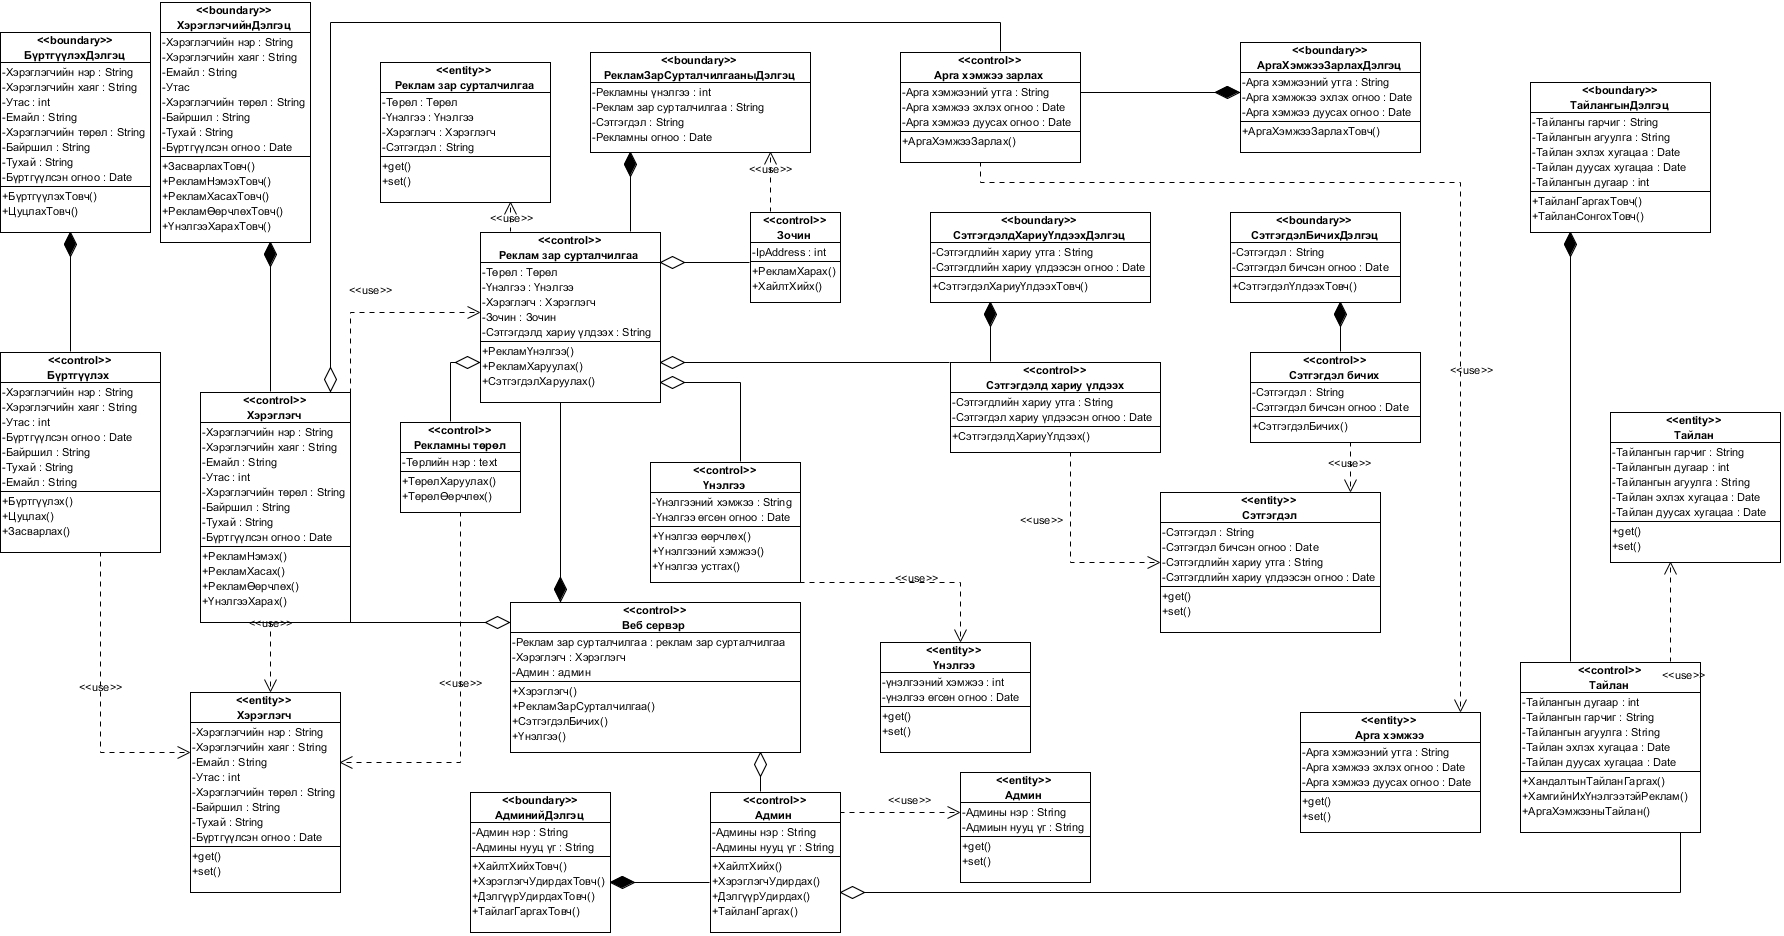
\includegraphics[angle=90,scale=0.34]{Diagrams/z_class}
		\caption[Зохиомжийн шатны класс диаграм]{Зохиомжийн шатны класс диаграм}
		\label{text}
	\end{figure}
\section{Дарааллын диаграм }
	\begin{figure}[!h]
		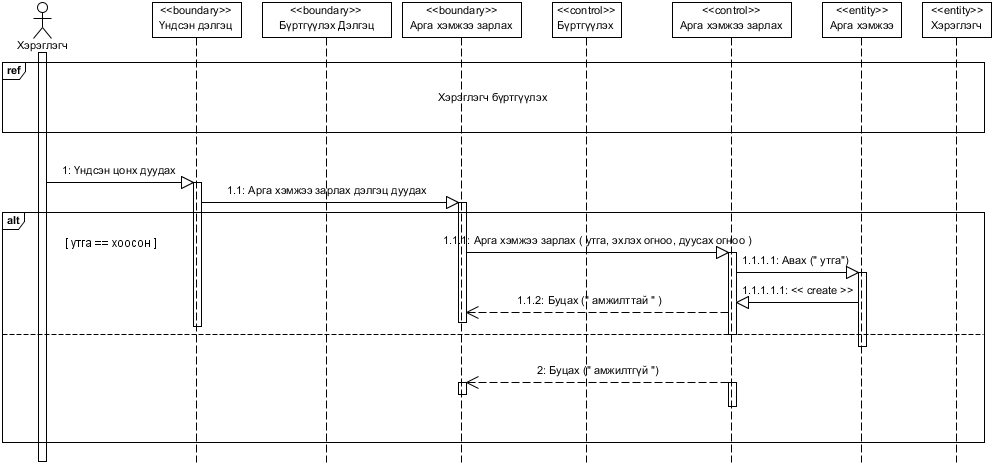
\includegraphics[scale=0.48]{Diagrams/event_s}
		\caption[Арга хэмжээ зарлах дарааллын диаграм]{Арга хэмжээ зарлах дарааллын диаграм}
		\label{text}
	\end{figure}

	\begin{figure}[!h]
		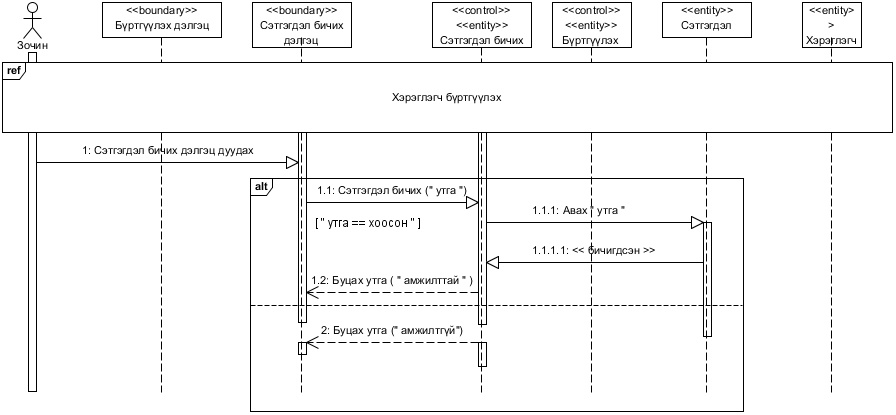
\includegraphics[scale=0.53]{Diagrams/comment_s}
		\caption[Сэтгэгдэл бичих дарааллын диаграм]{Сэтгэгдэл бичих дарааллын диаграм}
		\label{text}
	\end{figure}
	
	\begin{figure}[!h]
		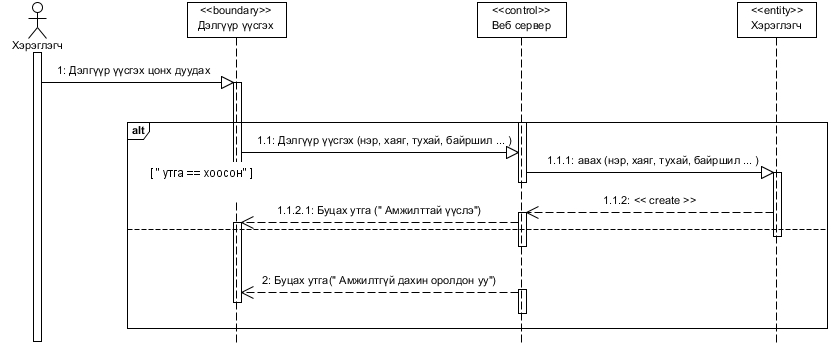
\includegraphics[scale=0.55]{Diagrams/create_s}
		\caption[Дэлгүүр үүсгэх дарааллын диаграм]{Дэлгүүр үүсгэх дарааллын диаграм}
		\label{text}
	\end{figure}


\section{Төлөвийн диаграм }
	\begin{figure}[!h]

		\includegraphics[scale=0.55]{Diagrams/state}
		\caption[Реклам зар сурталчилгаа удирдах төлөвийн диаграм]{Реклам зар сурталчилгаа удирдах төлөвийн диаграм}
		\label{text}
	\end{figure}

\section{Хэрэглэгчийн интерфейс }
	
\section{Тайлан, статистик үзүүлэлтийн загвар }
	
\section{Бүлгийн дүгнэлт}
	Зохиомжийн хэсэгт өгөгдлийн ерөнхий схем болон өмнөх шинжилгээний класс диаграм дээр үндэслэн зохиомжийн класс диаграм, дарааллын диаграмуудыг гаргасан. Хамгийн гол төлөвийн диаграмыг бас давхар гаргаж өгсөн байгаа. Бусад ижил төстэй томоохон сайтуудаас жишээ авч вебийн туршилтын загварыг гаргасан байгаа
\section{Ерөнхий дүгнэлт}
	Өнөө үед интернэтийн орчинд ажил, үйлчилгээгээ явуулах хувь хүн болон аж ахуйн нэгж албан байгууллагууд хурдацтай өсөн нэмэгдсэн билээ. Үүнийг ажиглан реклам зар сурталчилгааг интернэт дамжуулан хэрэглэгчид хүргэх нь одоогийн нийгэмд хамгийн зөв арга хэлбэр болоод байна. Энэхүү вебийг хийхэд дараах ажлуудыг хийж гүйцэтгэлээ:
	-	Тухайн вебийн талаар судалгаа явсан
	-	CodeIgniter framework –ийн судалгаа хийсэн
	-	Өгөгдлийн сан болон вебийн дотоод үйл ажиллагааг дүрслэн гаргасан
	-	Код бичих орчиноо бэлдэх, судалгаа шинжилгээ хийсэн
	

%\include{Chapters/Chapter4} 
%\include{Chapters/Chapter5}

%-------------------------------------------------------------------------------
%	THESIS CONTENT - APPENDICES
%-------------------------------------------------------------------------------

\appendix % Дараах "chapters" нь Хавсралт болохыг LaTex -д хэлэх

% Тезисийн бүлгүүдийг Appendices хавтаснаас бие даасан файл байдлаар оруулах

% Хавсралт A

%\chapter{Хавсралтын нэр} % Main appendix title

\label{AppendixA} % For referencing this appendix elsewhere, use \ref{AppendixA}

Хавсралтаа энд бичнэ.
%\include{Appendices/AppendixB}
%\include{Appendices/AppendixC}

%-------------------------------------------------------------------------------
%	BIBLIOGRAPHY
%-------------------------------------------------------------------------------
\defformat % Бүлгийн нэрийг оргиналь байдлаар хэвлэх

\addchaptertocentry{Ном зүй} % Ном зүйг гарчигт нэмэх

\printbibliography[heading=bibliography,title={Ном зүй}]

%-------------------------------------------------------------------------------
\end{document}
 